\section{MOSFET}

\subsection{PN Junction Diode}

\begin{itemize}
    \item \textbf{P-type}: Doped with acceptor impurities. Holes are majority carriers. Electrons are minority carriers.
    \item \textbf{N-type}: Doped with donor impurities. Electrons are majority carriers. Holes are minority carriers.
    \item \textbf{Depletion Region}: Region where the majority carriers are depleted. The region is charged. Depleted means the region is charged by the ions.
\end{itemize}

\subsection{Structure}

\begin{wrapfigure}{r}{0.5\textwidth}
    \centering
    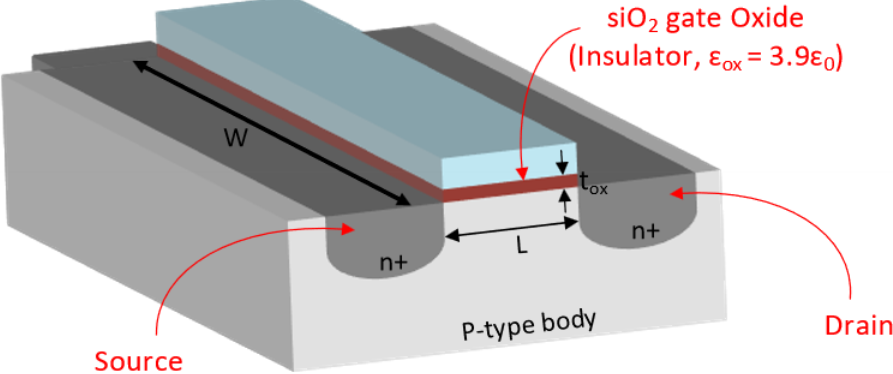
\includegraphics[scale=0.5]{images/MOSFET.png}
    \caption{MOSFET}
\end{wrapfigure}

The given image shows a MOSFET with P-type boday and N-type source and drain.
This is a NMOS transistor. Voltage applied to gate will allow current to flow
from source to drain.

\begin{itemize}
    \item \textbf{Polysilicon}: Silicon formed from many small silicon crystals.
    \item \textbf{Gate Oxide}: Insulating layer between the gate and the channel.
    \item Source and Drain are doped with N-type impurities. PMOS has P-type impurities
    with body as N-type.
    \item \textbf{Bulk}: Body of the transistor.
\end{itemize}

\subsubsection{Gate-body Structure}
\begin{figure}[h]
    \centering
    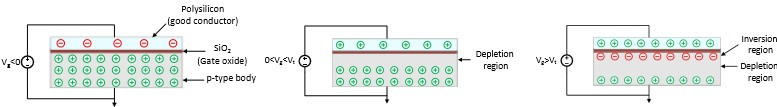
\includegraphics[scale=0.7]{images/MOS-device-theory.jpg}
    \caption{Gate-body Structure}
\end{figure}
\begin{enumerate}
    \item Accumulation mode: Gate voltage is negative or zero. Holes are attracted to the gate thus forming a channel. Low resistance.
    \item Depletion mode: Gate voltage is positive but less than threshold voltage. Holes are repelled from the gate. High resistance.
    \item Inversion mode: Gate voltage is greater than threshold voltage. Electrons are attracted to the gate thus forming holes at the body. Low resistance.
\end{enumerate}

\subsection{NMOS and PMOS}

Drain-Source current is controlled by the gate-source voltage.

\begin{figure}[h]
    \centering
    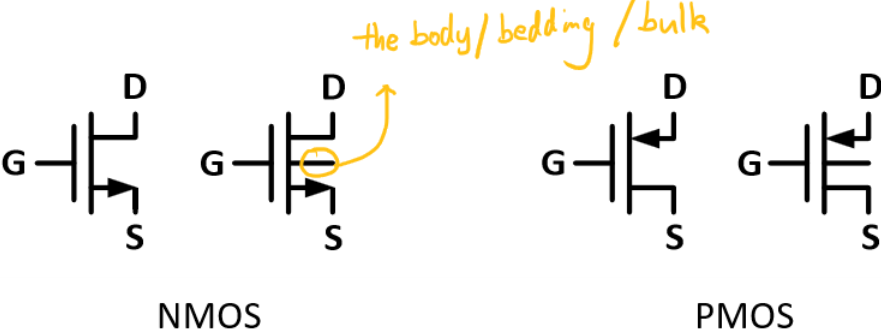
\includegraphics[scale=0.3]{images/NMOSandPMOS.png}
    \caption{MOSFET}
\end{figure}

\textbf{NMOS}: When $V_{GS} > V_{th}$, the transistor is on. When $V_{GS} < V_{th}$, the transistor is off.

\textbf{PMOS}: When $V_{GS} < V_{th}$, the transistor is on. When $V_{GS} > V_{th}$, the transistor is off.

\subsubsection{nMOS modes}

Source and drain are symmetric diffusion termninals. For nMOS, source is the termnial at lower voltage ($V_ds > 0$) 

\begin{figure}[h]
    \centering
    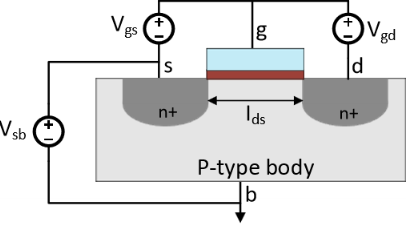
\includegraphics[scale=0.5]{images/nMOS.png}
    \caption{nMOS modes}
\end{figure}

\begin{itemize}
    \item Cutoff: $V_{GS} < V_{th}$, $I_{DS} = 0$. It is the depletion mode.
    \item Triode/Linear: $V_{GS} > V_{th}$, $V_{DS} < V_{GS} - V_{th}$. It is the linear mode.\begin{itemize}
        \item Conductivity is proportional to $V_{GS} - V_{th}$. The larger the $V_{GS} - V_{th}$, the larger the conductivity, the smaller the resistance.
        \item Current flow from D to S. Electrons flow from S to D.
    \end{itemize}
    \item Saturation: $V_{GS} > V_{th}$, $V_{DS} > V_{GS} - V_{th}$. It is the saturation mode.\begin{itemize}
        \item Channel is pinched off at the drain end. The current is independent of $V_{DS}$.
    \end{itemize}
\end{itemize}

\subsection{MOSFET Characteristics}

Carrier velocity is proportional to the electric field. $v_d = \mu_n E$. $\mu_n$ is the carrier mobility of the electrons.

Electric field is proportional to the voltage gradient. $E = \frac{dV}{dx}$. Can approximate as $E = \frac{V}{L}$ where $L$ is the length of the channel.

Thus time it takes for the electron to travel from source to drain is $t = \frac{L}{v_d} = \frac{L}{\mu_n E} = \frac{L^2}{\mu_n V}$.

$C_{ox}$ is the capacitance of the oxide layer. $C_{ox} = \frac{\epsilon_{ox}}{t_{ox}}$. With $W$ as the width of the channel, $L$ as the length of the channel, $C_{ox} = \frac{\epsilon_{ox} W L}{t_{ox}}$.

Let $\beta = \mu_n C_{ox} \frac{W}{L}$ be the gain factor. 

\begin{itemize}
    \item Cut-off: $I_{DS} = 0$.
    \item Triode: $I_{DS} = \beta (V_{GS} - V_{th} - \frac{V_{DS}}{2}) V_{DS}$.
    \item Saturation: $I_{DS} = \frac{\beta}{2} (V_{GS} - V_{th})^2$. independent of $V_{DS}$.
\end{itemize}

For a fixed $V_ds$ and $V_{GS} > V_{th}$, the current is proportional to:\begin{itemize}
    \item $L$: The length of the channel. The longer the channel, the longer the time it takes for the electron to travel from source to drain.
    \item $W$: The width of the channel. The wider the channel, the more electrons can flow through.
    \item $V_{th}$: The threshold voltage. The larger the threshold voltage, the larger the current.
    \item $\epsilon_{ox}$: The permittivity of the oxide layer. The larger the permittivity, the larger the current.
    \item $t_{ox}$: The thickness of the oxide layer. The thinner the oxide layer, the larger the current.
    \item $\mu_n$: The carrier mobility of the electrons. The larger the carrier mobility, the larger the current.\begin{itemize}
        \item $\mu_n = 500cm^2/V \cdot sec \approx 2.5 \mu_p$. $\mu_p = 180cm^2/V \cdot sec$.
        \item Thus need to increase the size of pmos to match the current of nmos.
    \end{itemize}
\end{itemize}

For small $V_{DS}$, the transistor is viewed as a linear resitor. 

$R_{on} = \frac{1}{\beta (V_{GS} - V_{th})}$.

\subsubsection{Region of Operation}

\begin{figure}[h]
    \centering
    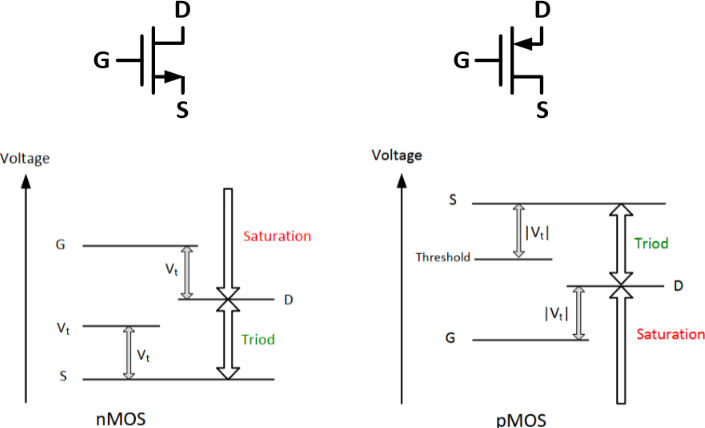
\includegraphics[scale=1]{images/MOS_relative_voltage.png}
    \caption{Region of Operation}
\end{figure}